\documentclass[presentation]{beamer}

\usepackage{tikz}
\usetikzlibrary{positioning,calc,matrix}
\usetikzlibrary{shapes.geometric}
\usetikzlibrary{backgrounds}% only to show the bounding box
\usepackage{pgf}
\usepackage{pgfplots}
\pgfplotsset{compat=1.13}
\usepackage{pgfplotstable}
\usepackage{appendixnumberbeamer}
\usepackage{amsmath}
\usepackage{pifont}
\newcommand{\cmark}{\ding{51}}
\newcommand{\xmark}{\ding{55}}
\DeclareMathOperator{\tr}{tr}
\DeclareMathOperator{\grad}{grad}
\let\div\relax
\DeclareMathOperator{\div}{div}
\DeclareMathOperator{\curl}{curl}
\date{6th July 2017}
\usetheme{metropolis}
\metroset{progressbar=frametitle}

\renewcommand{\vec}[1]{\ensuremath{\boldsymbol{#1}}}
\newcommand{\ddt}[1]{\frac{\partial #1}{\partial t}}
\newcommand{\zhat}{\hat{\vec{z}}}
\newcommand{\W}{\ensuremath{\mathbb{W}}}

\newcommand{\inner}[1]{\left\langle #1 \right \rangle}

\newcommand{\KSP}[2]{\ensuremath{\mathcal{K}\left(#1, \mathbb{#2}\right)}}
\newcommand{\ksp}[1]{\KSP{#1}{#1}}

\newcommand{\highlight}[1]{\colorbox{red!20}{\color{black} #1}}
\newcommand{\arxivlink}[2]{%
  \href{http://www.arxiv.org/abs/#1}%
  {\texttt{arXiv:\,#1\,[#2]}}%
}
\newcommand{\doilink}[1]{%
  \href{http://dx.doi.org/#1}%
  {\texttt{doi:\,#1}{}}%
}

\author{Lawrence Mitchell\inst{1,*}}
\institute{
\inst{1}Departments of Computing and Mathematics, Imperial College
London

\inst{*}\texttt{lawrence.mitchell@imperial.ac.uk}
}

\graphicspath{{./\jobname.figures/}{../pictures/}}

\usepackage[url=false,
            doi=true,
            isbn=false,
            style=authoryear,
            giveninits=true,
            uniquename=init,
            backend=biber]{biblatex}

\setbeamertemplate{bibliography item}{}

\renewcommand{\bibfont}{\fontsize{7}{7}\selectfont}
\addbibresource{references.bib}

\setlength{\bibitemsep}{1ex}
\setlength{\fboxsep}{1pt}

\renewbibmacro{in:}{}
\DeclareFieldFormat[article]{volume}{\textbf{#1}}
\DeclareFieldFormat{doi}{%
  doi\addcolon%
  {\scriptsize\ifhyperref{\href{http://dx.doi.org/#1}{\nolinkurl{#1}}}
    {\nolinkurl{#1}}}}
\AtEveryBibitem{%
\clearfield{pages}%
\clearfield{issue}%
\clearfield{number}%
}

\usepackage{minted}
\RecustomVerbatimEnvironment{Verbatim}{BVerbatim}{}

\title{Symbolic numerical computing}
\begin{document}
\begin{frame}[plain,noframenumbering]
  \maketitle
  \begin{tikzpicture}[remember picture,overlay]
    \node[at=(current page.south west), anchor=south west] {
\includegraphics[height=0.9cm]{epsrc-logo}};
  \node[at=(current page.south east), anchor=south east] {\includegraphics[height=0.9cm]{imperial-two-tone}};
\end{tikzpicture}
\end{frame}

\begin{frame}[t]
  \frametitle{A problem}
  \begin{itemize}
  \item Computational simulation underpins much of modern science and
    engineering.
  \item Simulation models are ever more complex.
  \item The extra computational effort used to be offset by increased
    hardware performance \ldots
  \end{itemize}
  \begin{columns}
    \begin{column}{0.95\paperwidth}
      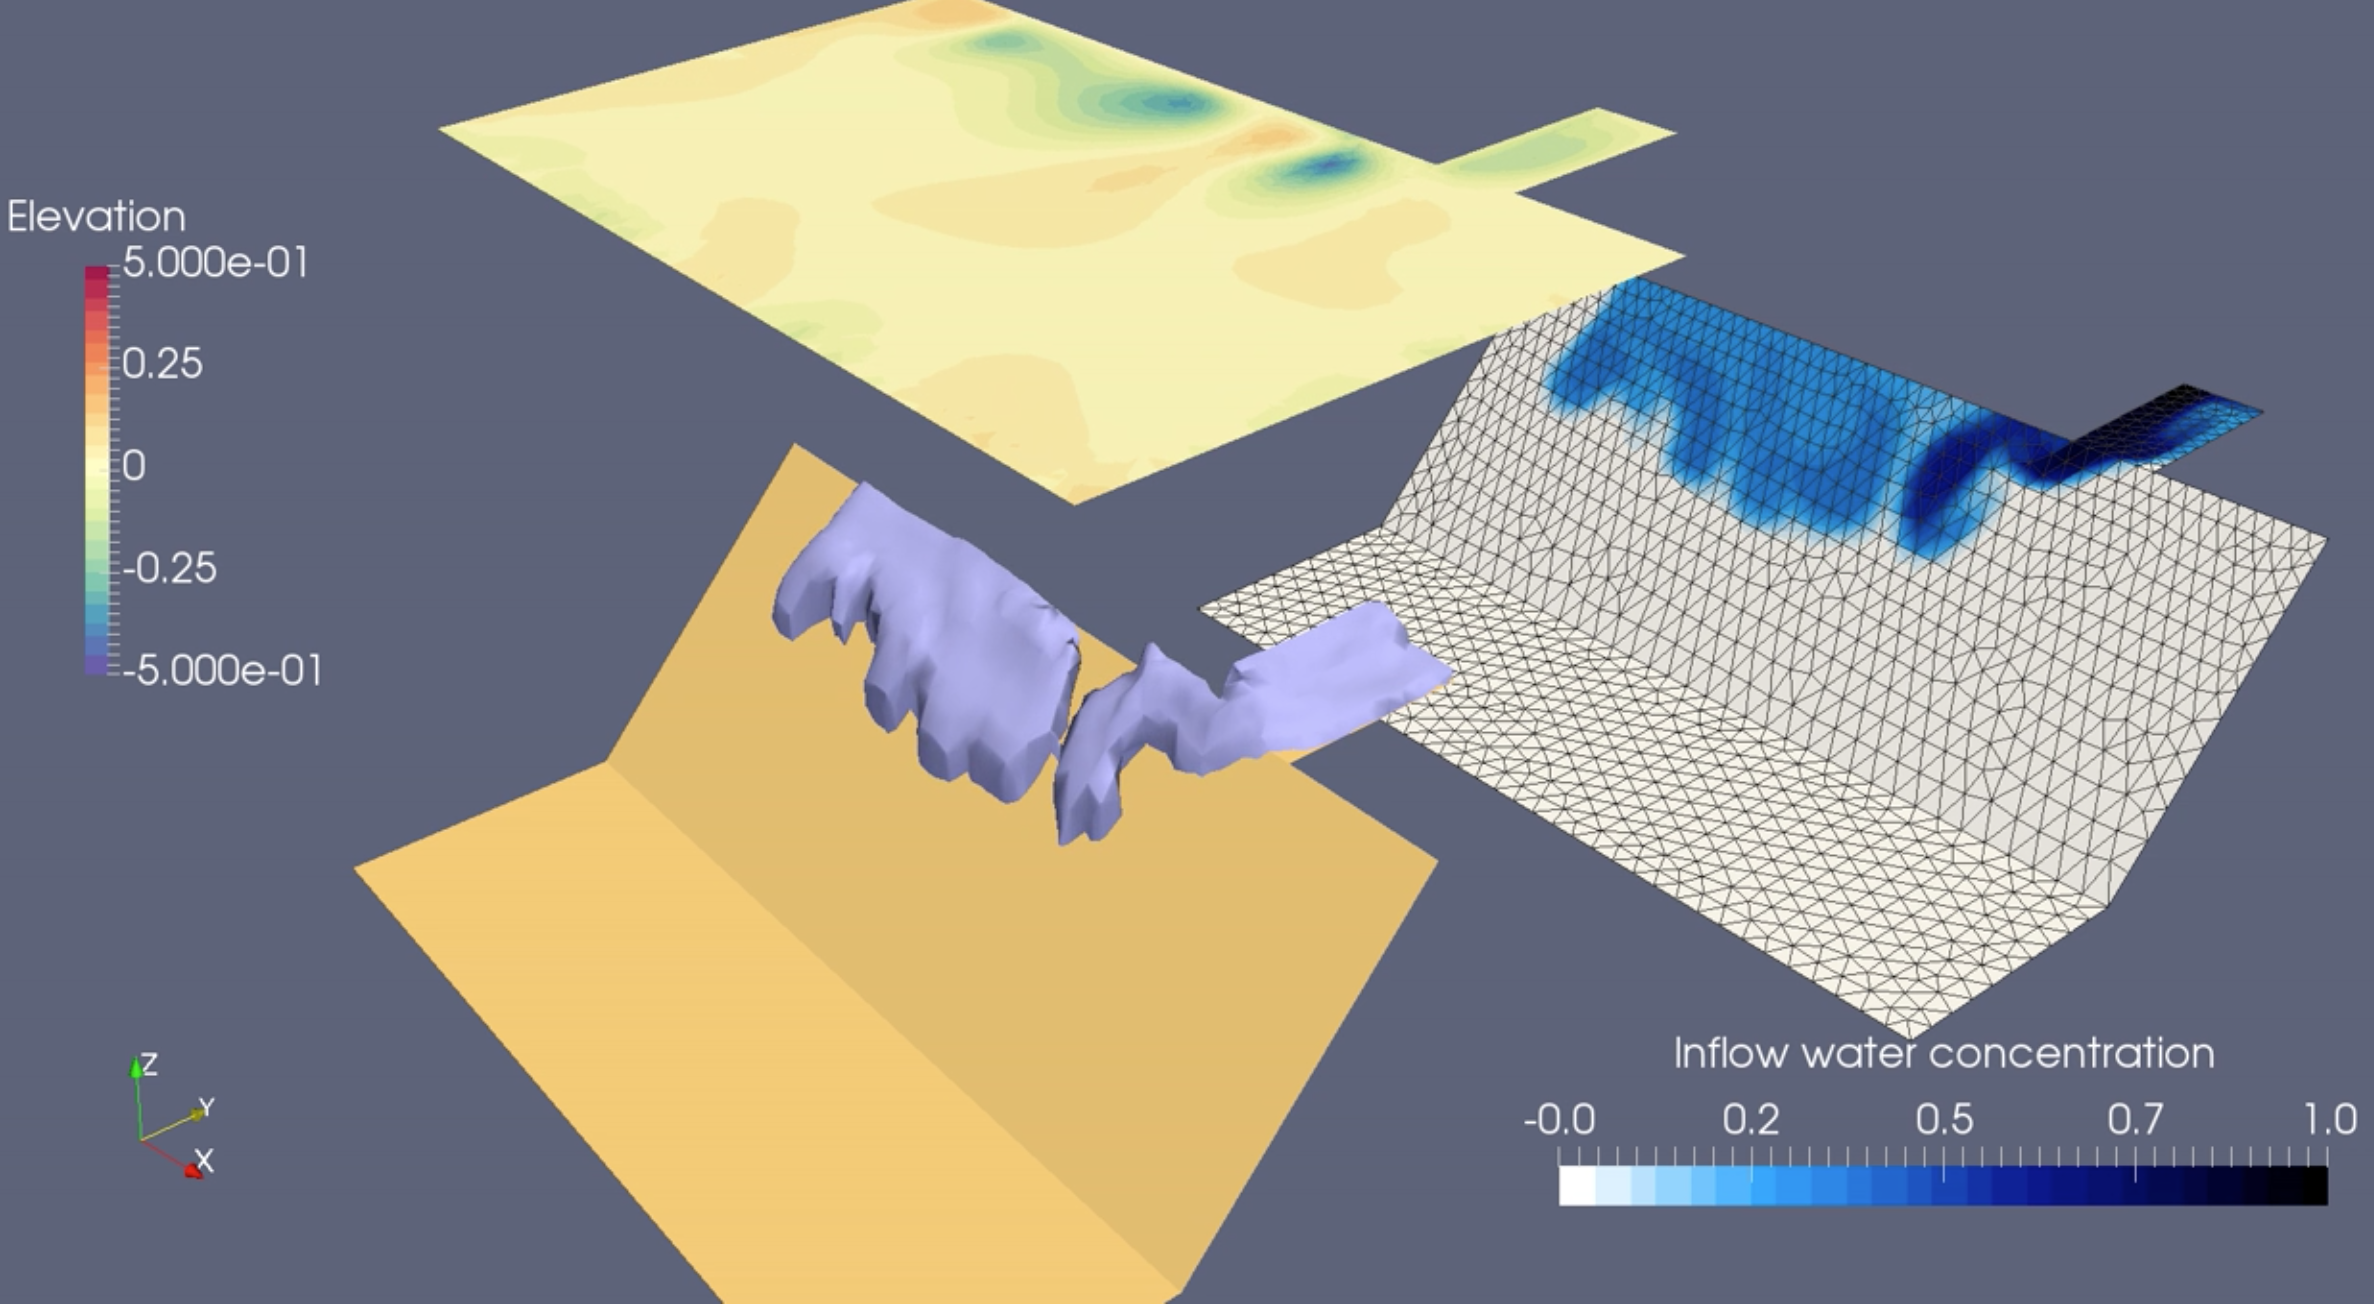
\includegraphics[height=4cm]{dome-entrainment}\hfill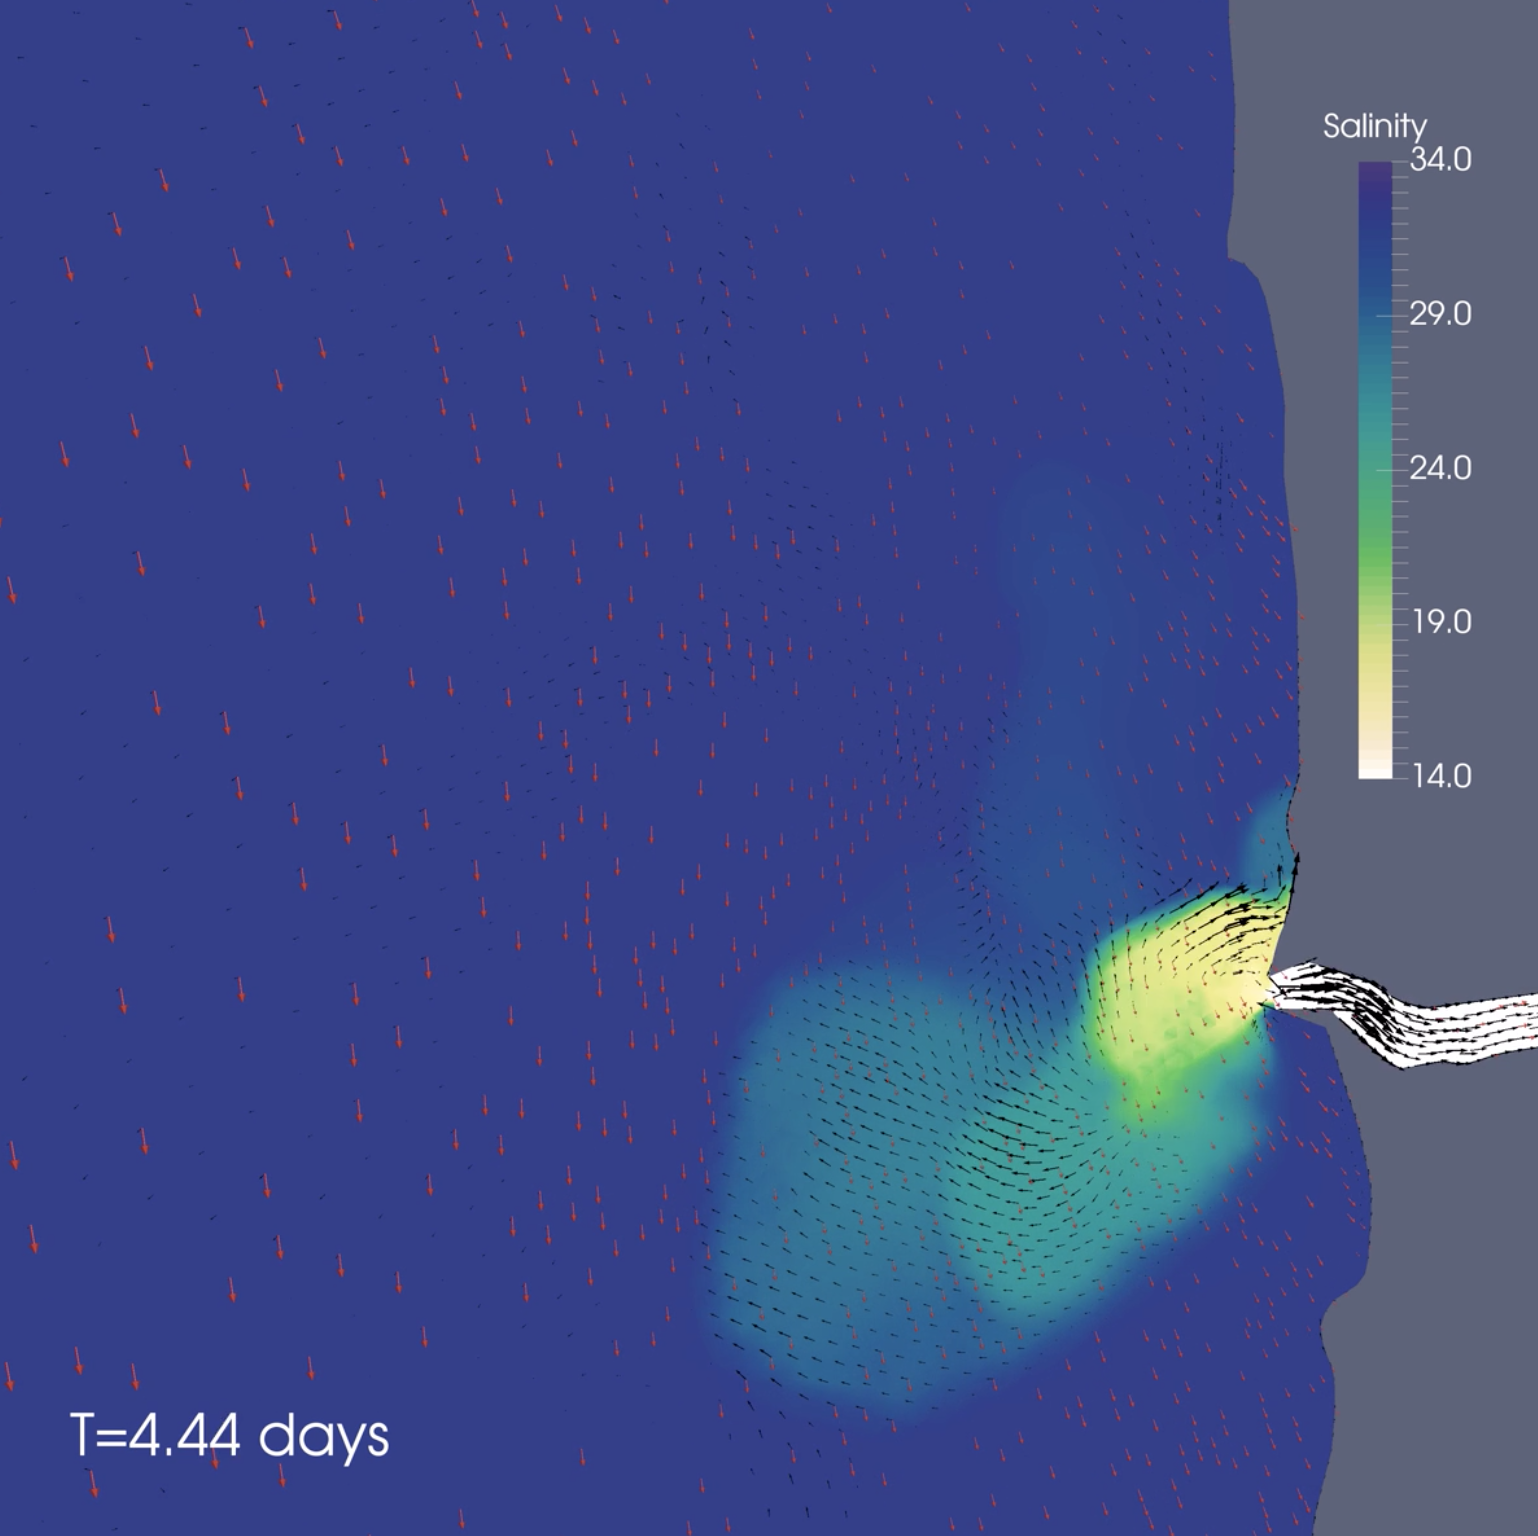
\includegraphics[height=4cm]{columbia-plume}
    \end{column}
  \end{columns}
\end{frame}

\begin{frame}
  \frametitle{The free lunch finished a long time ago}
    \begin{center}
      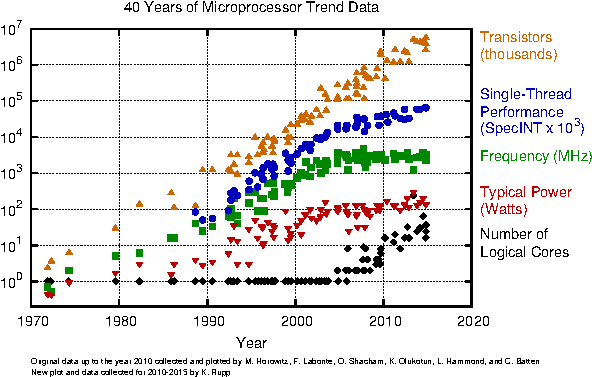
\includegraphics[height=0.6\textheight]{processor-trends}
    \end{center}
    \vspace{-2em}
    \begin{flushright}
      {\tiny Figure courtesy Karl Rupp (CC-BY 4.0) \url{https://www.karlrupp.net/2015/06/40-years-of-microprocessor-trend-data/}}
    \end{flushright}
  \begin{itemize}
  \item Today's simulation models will run probably \emph{slower}, not faster, on
    tomorrow's hardware.
  \end{itemize}
\end{frame}

\begin{frame}
  \frametitle{What are the challenges?}
  \begin{itemize}
  \item Simulation software needs to exploit \emph{fine-grained}
    parallelism.
  \item Most code intimately intertwines the numerical algorithm with
    its \emph{implementation}.
  \item To apply program transformations, we have to unpick,
    understand, and reimplement.
  \end{itemize}
\end{frame}

\begin{frame}[fragile]
  \frametitle{Exploiting mathematical abstractions}
  Compute $y \leftarrow \nabla^2 x$ using finite differences.
  \begin{equation*}
    y_{i,j} = x_{i-1, j} + x_{i+1, j} + x_{i, j-1} + x_{i, j+1} - 4x_{i,j}    
  \end{equation*}
  \begin{overlayarea}{\textwidth}{0.8\textheight}
  \begin{onlyenv}<1>
    \begin{block}{Before 1953}
\begin{minted}[fontsize=\tiny]{asm}
        ...
        faddp   %st, %st(1)
        movl    -8(%ebp), %edx
        movl    %edx, %eax
        sall    $2, %eax
        addl    %edx, %eax
        leal    0(,%eax,4), %edx
        addl    %edx, %eax
        sall    $2, %eax
        movl    %eax, %edx
        movl    -4(%ebp), %eax
        addl    %edx, %eax
        subl    $101, %eax
        flds    x.3305(,%eax,4)
        flds    .LC0
        fmulp   %st, %st(1)
        faddp   %st, %st(1)
        fstps   y.3307(,%ecx,4)
        ...
\end{minted}
    \end{block}
  \end{onlyenv}
  \begin{onlyenv}<2->
    \begin{block}{1953--present: FORmula TRANslation}
\begin{minted}[fontsize=\tiny]{fortran}
      PROGRAM MAIN
      PARAMETER (N=100)
      REAL X(N,N), Y(N,N)
      DO 10 J=2,N-1
         DO 20 I=2,N-1
            Y(I,J)=X(I-1,J)+X(I+1,J)+X(I,J-1)+X(I,J+1)+4*X(I,J)
 20      CONTINUE
 10   CONTINUE
      DO 30 I=1,N
         Y(I,1) = 0.0
         Y(I,N) = 0.0
         Y(1,I) = 0.0
         Y(N,I) = 0.0
 30   CONTINUE
      END
\end{minted}
    \end{block}
  \end{onlyenv}
  \end{overlayarea}
\end{frame}

\begin{frame}
  \frametitle{Firedrake \url{www.firedrakeproject.org}}

  \begin{quote}
    {\normalfont [\ldots]} an automated system for the solution of partial
    differential equations using the finite element method.
  \end{quote}

  \begin{itemize}
  \item Written in Python.
  \item Finite element problems specified with \emph{embedded} domain
    specific language.
  \item \emph{Runtime} compilation to low-level (C) code.
  \item Explicitly \emph{data parallel}: don't worry about MPI.
  \end{itemize}

  \begin{flushright}
    {\scriptsize F.~Rathgeber, D.A.~Ham, \textbf{LM}, M.~Lange,
      F.~Luporini, A.T.T.~McRae, G.-T.~Bercea, G.R.~Markall,
      P.H.J.~Kelly. ACM Transactions on Mathematical Software,
      2016. \arxivlink{1501.01809}{cs.MS}}
  \end{flushright}
\end{frame}

\begin{frame}
  \frametitle{Finite element crash course}
  \begin{columns}
    \begin{column}{0.5\textwidth}
      \begin{align*}
        F(u) &= 0 \text{ in $\Omega$}\\
        u &= g \text{ on $\Gamma_1$}\\
        \frac{\partial u}{\partial n} &= h \text{ on $\Gamma_2$}
      \end{align*}
    \end{column}
    \begin{column}{0.5\textwidth}
      \begin{tikzpicture}
        \draw[very thick, line cap=rect] (0,0) -- (5, 0) (0, 0) arc
        (180:360:2.5);
      \end{tikzpicture}
    \end{column}
  \end{columns}

  Seek \emph{weak} solution in some space of functions $V(\Omega)$.

  Now we need to solve the (infinite dimensional) problem, find $u\in V$ s.t.
  \begin{equation*}
    \int_\Omega \!F(u) v\, \text{d}x = 0 \quad \forall\, v \in V
  \end{equation*}
\end{frame}
\begin{frame}
  \frametitle{Finite element crash course}
  \begin{columns}
    \begin{column}{0.5\textwidth}
      Choose a \emph{triangulation}, $\mathcal{T}$, for $\Omega$, and
      a finite dimensional subspace $V_h \subset V$.  Then
    \end{column}
    \begin{column}{0.5\textwidth}
        \begin{tikzpicture}
          \path (0,0) arc[radius=2.5, start angle=180, end angle=360]
          node[name=E,pos=0,swap] {} node[name=F,pos=0.25,swap] {}
          node[name=G,pos=0.5,swap] {} node[name=H,pos=0.82,swap] {}
          node[name=I,pos=1,swap] {}; \node (A) at (2.5, 0) {}; \node
          (B) at (1.4, -0.7) {}; \node (C) at (3.4, -1.2) {}; \node
          (D) at (1.8, -1.5) {};

          \draw[color=black, very thick, line cap=butt, line
          join=round] (E.center) -- (A.center) -- (I.center) --
          (H.center) -- (G.center) -- (F.center) -- (E.center) --
          cycle; \draw[color=black, very thick, line cap=butt, line
          join=round] (E.center) -- (B.center) -- (D.center) --
          (F.center) -- (B.center); \draw[color=black, very thick,
          line cap=butt, line join=round] (G.center) -- (D.center) --
          (C.center) -- (G.center); \draw[color=black, very thick,
          line cap=butt, line join=round] (B.center) -- (A.center) --
          (C.center) -- (B.center); \draw[color=black, very thick,
          line cap=butt, line join=round] (H.center) -- (C.center) --
          (I.center);
        \end{tikzpicture}
    \end{column}
  \end{columns}

  \begin{equation*}
    \int_\Omega \! F(u) v\,\text{d}x \approx \sum_{e\in\mathcal{T}}
    \int_e\! F(u_h)v_h \,\text{d}x.
  \end{equation*}

  We can perform the remaining integral with numerical quadrature
  \begin{equation*}
    \int_e F(u_h)v_h\,\text{d}x \approx \sum_q w_q F(u_h(q)) v_h(q).
  \end{equation*}
\end{frame}

\begin{frame}[fragile]
  \frametitle{Fit to the mathematics}
  \begin{itemize}
  \item Firedrake builds on, and extends, embedded DSLs developed in
    the FEniCS project.
  \item Particularly, the \emph{Unified Form Language} \parencite{Alnaes:2014} to
    specify variational forms
  \item Synthesise efficient implementation from symbolic description
    + problem-specific data.
  \end{itemize}
  \begin{columns}
    \begin{column}{0.4\textwidth}
      \begin{equation*}
        \int_\Omega \nabla u \cdot \nabla v\,\text{d}x
      \end{equation*}
    \end{column}
    \hspace{-3em}
    \begin{column}{0.6\textwidth}
\begin{minted}[fontsize=\scriptsize]{python}
V = FiniteElement("Lagrange", triangle, 1)
u = TrialFunction(V)
v = TestFunction(V)
a = dot(grad(u), grad(v))*dx
\end{minted}
    \end{column}
  \end{columns}
\end{frame}

\begin{frame}[fragile]
  \frametitle{A compiler for finite elements}
  A \emph{form compiler} translates UFL into
  low-level (C/C++/...) code for performing an element integral.
  \begin{flushright}
    {\scriptsize M.~Homolya, \textbf{LM}, F.~Luporini, D.A.~Ham. \arxivlink{1705.03667}{cs.MS}}
  \end{flushright}
  \begin{overlayarea}{\textwidth}{0.8\textheight}
  \begin{onlyenv}<1> 
    \begin{itemize}
    \item Element integral
      \begin{columns}
        \begin{column}{0.4\textwidth}
          \begin{equation*}
            \int_e \nabla u \cdot \nabla v\,\text{d}x
          \end{equation*}
        \end{column}
        \hspace{-3em}
        \begin{column}{0.6\textwidth}
\begin{minted}[fontsize=\scriptsize]{python}
V = FiniteElement("Lagrange", triangle, 1)
u = TrialFunction(V)
v = TestFunction(V)
a = dot(grad(u), grad(v))*dx
\end{minted}
        \end{column}
      \end{columns}
    \item Is transformed to a tensor algebra expression
      {\small \begin{equation*}
    \sum_q w_q \left| d \right| \sum_{i_5} \left( \sum_{i_3}
      K_{i_3,i_5} \begin{bmatrix}
        E^{(1)}_{q,k} & E^{(2)}_{q,k}
      \end{bmatrix}_{i_3} \right)
    \left( \sum_{i_4} K_{i_4,i_5} \begin{bmatrix}
        E^{(1)}_{q,j} & E^{(2)}_{q,j}
      \end{bmatrix}_{i_4} \right)
  \end{equation*}}
    \item Compiler passes aim to minimise FLOPs required to evaluate
      this expression.
    \end{itemize}
  \end{onlyenv}
  \begin{onlyenv}<2>
    \begin{columns}
      \begin{column}{0.5\textwidth}
\begin{minted}[fontsize=\tiny]{c}
void cell_integral(double A[3][3],
                   double coords[3][2]) {
  static const double t10[3] = {...};
  static const double t12[3] = {...};
  double t13[3];
  double t14[3];
  double t0 = (-1 * coords[0][1]);
  double t1 = (t0 + coords[1][1]);
  double t2 = (-1 * coords[0][0]);
  double t3 = (t2 + coords[1][0]);
  double t4 = (t0 + coords[2][1]);
  double t5 = (t2 + coords[2][0]);
  double t6 = ((t3 * t4) + (-1 * (t5 * t1)));
  double t7 = ((-1 * t1) / t6);
  double t8 = (t4 / t6);
  double t9 = (t3 / t6);
  double t11 = ((-1 * t5) / t6);
\end{minted}
      \end{column}
      \begin{column}{0.5\textwidth}
\begin{minted}[fontsize=\tiny]{c}
  for (int k0 = 0; k0 < 3; k0++) {
    t13[k0] = (t11 * t12[k0]) + (t9 * t10[k0]);
    t14[k0] = (t8 * t12[k0]) + (t7 * t10[k0]);
  }
  double t15 = (0.5 * fabs(t6));
  for (int j0 = 0; j0 < 3; j0++) {
    double t16 = ((t11 * t12[j0])
                  + (t9 * t10[j0]));
    double t17 = ((t8 * t12[j0])
                  + (t7 * t10[j0]));
    for (int k0 = 0; k0 < 3; k0++) {
      A[j0][k0] += t15 * ((t17 * t14[k0])
                          + (t16 * t13[k0]));
    }
  }
}
\end{minted}
      \end{column}
    \end{columns}
  \end{onlyenv}
  \end{overlayarea}
\end{frame}

\begin{frame}
  \frametitle{FLOP-optimal tensor contractions}
  An important class of finite elements uses \emph{tensor product}
  basis functions
  \begin{equation*}
    \phi_{i,q} := \phi_{(j,k),(p,r)} = \varphi_{j,p}\varphi_{k,r}
  \end{equation*}

  This gives opportunities for factorisation of index-invariant
  expressions
  \begin{align*}
    \mathcal{F}_q &= \sum_i \phi_{i,q} f_i  \quad \text{needs
                    $\mathcal{O}(p^{2d})$ ops}\\
    \mathcal{F}_{(p,r)} &= \sum_{j,k} \phi_{(j,k),(p,r)} f_{j,k} = \sum_{j,k} \varphi_{j,p}\varphi_{k,r} f_{j,k} \\
                        &= \sum_j \varphi_{j,p} \sum_k \varphi_{k,r}
                          f_{j,k} \quad \text{needs
                          $\mathcal{O}(dp^{d+1})$ ops}
  \end{align*}
  \begin{flushright}
    {\scriptsize M.~Homolya, R.C.~Kirby, D.A.~Ham. \arxivlink{1711.02473}{cs.MS}}
  \end{flushright}
\end{frame}

\begin{frame}[fragile]
  \frametitle{Automated, not just for toy problems}
  \begin{columns}
    \begin{column}{0.5\textwidth}
      \begin{block}{}
        Find $u \in V \subset H(\curl)$ s.t.
        {\scriptsize \begin{equation*}
          \int\!\!\curl u \cdot \curl v \,\text{d}x = \int\!\!B\cdot
          v\,\text{d}x \quad \forall v \in V.
        \end{equation*}}
\begin{minted}[fontsize=\tiny,mathescape]{python}
NCE = FiniteElement("NCE", hexahedron, degree)
Q = VectorElement("Q", hexahedron, degree)
u = Coefficient(NCE) # Solution in $H(\curl)$
B = Coefficient(Q)   # Coefficient in $H^1$
v = TestFunction(NCE)
F = (dot(curl(u), curl(v)) - dot(B, v))*dx
\end{minted}
    \end{block}
    {\fontsize{9}{9}\selectfont
      \begin{itemize}
        \item<2-> TSFC obtains optimal \emph{complexity} evaluation
        \item<2-> In progress: is the constant factor good?
        \item<2-> Much still to be done in terms of vectorisation.
        \end{itemize}
      }
    \end{column}
  \begin{column}{0.6\textwidth}
  \begin{center}
    \begin{tikzpicture}[scale=0.9]
      \begin{loglogaxis}[name=plot, small, title=FLOPs to evaluate $F$,
        xlabel=Polynomial degree,
        ylabel=FLOPs, xtick={1,2,4,8,16,32},
        xticklabels={$1$,$2$,$4$,$8$,$16$,$32$}, axis lines=left, axis
        line style={-}, log basis x=2,
        legend entries={Na\"ive (no sum fact), With sum factorisation},
        legend style={at={(0.5,-0.3)},anchor=north,draw=none}]
        \pgfplotstableread[row sep=crcr]{
degree flops_vanilla flops_opt\\
1 9.78100e+03 6.48100e+03\\
2 1.05624e+05 2.78280e+04\\
3 6.04110e+05 7.50860e+04\\
4 2.36102e+06 1.63395e+05\\
5 7.20724e+06 3.09060e+05\\
6 1.85105e+07 5.33483e+05\\
7 4.18644e+07 8.60322e+05\\
8 8.59101e+07 1.31626e+06\\
9 1.63287e+08 1.93100e+06\\
10 2.91712e+08 2.73728e+06\\
11 4.95190e+08 3.77084e+06\\
12 8.05352e+08 5.07047e+06\\
13 1.26293e+09 6.67796e+06\\
14 1.91933e+09 8.63816e+06\\
15 2.83841e+09 1.09989e+07\\
16 4.09829e+09 1.38110e+07\\
17 5.79335e+09 1.71285e+07\\
18 8.03637e+09 2.10082e+07\\
19 1.09608e+10 2.55101e+07\\
20 1.47229e+10 3.06972e+07\\
21 1.95048e+10 3.66353e+07\\
22 2.55164e+10 4.33937e+07\\
23 3.29987e+10 5.10443e+07\\
24 4.22266e+10 5.96621e+07\\
25 5.35115e+10 6.93253e+07\\
26 6.72053e+10 8.01150e+07\\
27 8.37026e+10 9.21153e+07\\
28 1.03445e+11 1.05413e+08\\
29 1.26924e+11 1.20099e+08\\
30 1.54686e+11 1.36267e+08\\
31 1.87334e+11 1.54011e+08\\
32 2.25533e+11 1.73433e+08\\
}\data; \pgfplotstableset{create on use/vanilla/.style={create
            col/expr={1e3*pow(\thisrow{degree},6)}}};
        \pgfplotstableset{create on use/spectral/.style={create
            col/expr={5e2*pow(\thisrow{degree},4)}}};
  
        \addplot+[mark=none, color=black, line width=1.5pt] table
        [x=degree,y=flops_vanilla] \data; \addplot+[mark=none,
        color=black, dashed, line width=1.5pt] table
        [x=degree,y=flops_opt] \data; \addplot+[mark=none, color=black,
        dotted, line width=1pt] table [x=degree,y=vanilla] \data
        coordinate [pos=0.67] (A); \node at (A) [anchor=south east]
        {$\mathcal{O}(p^6)$}; \addplot+[mark=none, color=black,
        dotted, line width=1pt] table [x=degree,y=spectral] \data
        coordinate [pos=0.67] (B); \node at (B) [anchor=north west]
        {$\mathcal{O}(p^4)$};
      \end{loglogaxis}
    \end{tikzpicture}
  \end{center}    
  \end{column}
  \end{columns}  
\end{frame}

\begin{frame}
  \frametitle{Future directions}
  \begin{itemize}
  \item Vectorisation and code generation for SIMD/GPUs
  \item Requires an intermediate representation for element kernels,
    and loop over elements.
    \begin{flushright}
      {\scriptsize with Andreas Kl\"ockner (UIUC), TJ Sun, and Paul
        Kelly}
    \end{flushright}
    \item Capture slightly wider class of tensor algebra
    \item Many finite element schemes require element-local
      manipulations (e.g. inverses, matrix-matrix products)
      \begin{flushright}
        {\scriptsize with Thomas Gibson, David Ham, and Colin Cotter.}
      \end{flushright}
    \end{itemize}
\end{frame}

\begin{frame}
  \frametitle{High performance solvers}
  \begin{itemize}
  \item In most cases, after discretising a PDE, we need to
    \emph{solve} a (non)linear problem.
  \item Designing robust, scalable solvers is a vast area of research
    in applied mathematics.
  \item Papers often only present (serial) proof of concept.
  \item Need low-cost means of comparing different options.
  \end{itemize}
  \begin{block}{Idea}
    Extend Firedrake's DSL to encompass building blocks of
    multi-level and domain decomposition solvers.
    \begin{flushright}
      {\scriptsize with Rob Kirby (Baylor), and Matt Knepley (Buffalo)}
    \end{flushright}
  \end{block}
\end{frame}

\begin{frame}
  \frametitle{An example that works: block preconditioning}
  \begin{itemize}
  \item Block system
    \begin{equation*}
    \begin{bmatrix}
      A & B^T \\
      C & 0
    \end{bmatrix}
  \end{equation*}
  \item $A$ sparse, but $A^{-1}$ dense
  \item Use iterative methods, with preconditioner
  \item For example  \begin{equation*}
      T = \begin{bmatrix}
        A & 0 \\
        0 & S := C A^{-1} B^T
      \end{bmatrix}^{-1}
      \begin{bmatrix}
        A & B^T \\
        C & 0
      \end{bmatrix}
    \end{equation*}
  \item Game is to find a good approximation to $S^{-1}$.
  \item Often, this will not be some function of $A$, $B^T$, and $C$.
  \end{itemize}
\end{frame}

\begin{frame}
  \frametitle{Block solvers in Firedrake}
  \begin{itemize}
  \item Provide mechanism for plugging in approximations to
    $S^{-1}$, in reusable, composable way.
  \item After all, they ``just'' need more matrices.
  \item Separates mathematics (what) from implementation (how).
  \item Your ``proof of concept'' solver becomes both scalable and
    high performance, transparently ports to new architectures with
    Firedrake.
    \begin{flushright}
      {\scriptsize R.C.~Kirby and \textbf{LM}. SIAM Journal on Scientific Software,
        2018. \arxivlink{1706.01346}{cs.MS}.}
    \end{flushright}
  \end{itemize}
\end{frame}

\begin{frame}
  \frametitle{Conclusions}
  \begin{itemize}
  \item DSLs are more than a pretty face.
  \item Offer many opportunities for employing ``traditional''
    computer science in new settings.  Productive interdisciplinary
    research!
  \item Much still to do:
    \begin{itemize}
    \item compiler development: vectorisation, GPUs, more tensor
      algebra.
    \item custom solver specification for ``hard'' problems: domain
      decomposition, better multigrid, \dots.
    \end{itemize}
  \end{itemize}
\end{frame}

\section{Lecture excerpt}

% \begin{frame}
%   \frametitle{Overview}
%   \begin{itemize}
%   \item Some cautionary tales
%   \item How computers represent numbers
%   \item Difficulties due to finite range/precision
%   \item Numerical \emph{conditioning} and how to tell when you have
%     nonsense answers
%   \end{itemize}
% \end{frame}

% \begin{frame}[plain,t]
%   \begin{flushright}
%       \tiny CC BY-SA 3.0
%       \url{https://commons.wikimedia.org/wiki/File:Boeing_787_Roll-out.jpg}
%   \end{flushright}
%   \begin{tikzpicture}[remember picture, overlay]
%     \node[at=(current page.center)] (dreamliner)
%     {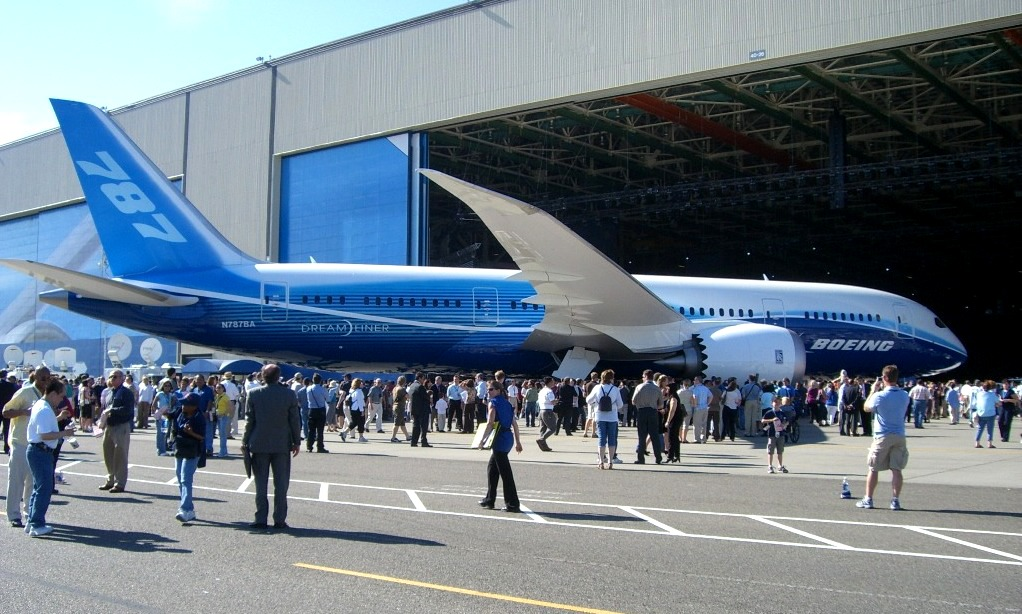
\includegraphics[width=\paperwidth]{dreamliner}};
%     \uncover<2->{\node [below right=1cm of dreamliner.north west, anchor=north west]
%       {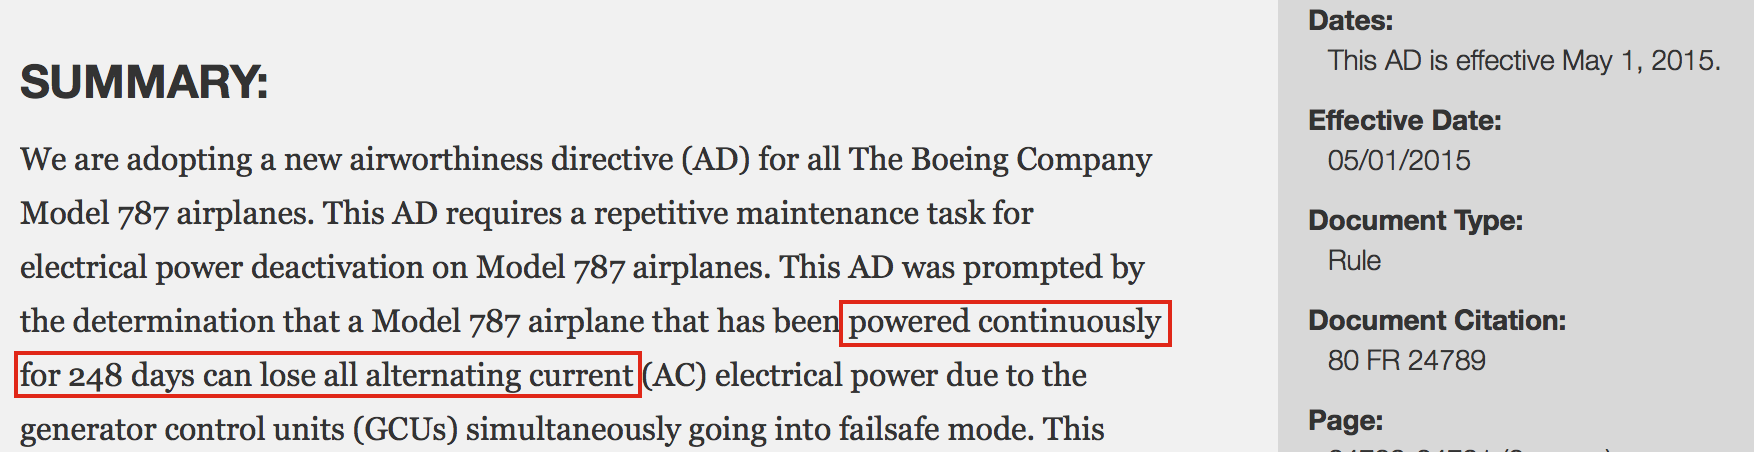
\includegraphics[width=1\framewidth]{dreamliner-bug-2015}};}
%     \uncover<3->{\node [above left=1cm of dreamliner.south east, anchor=south east]
%       {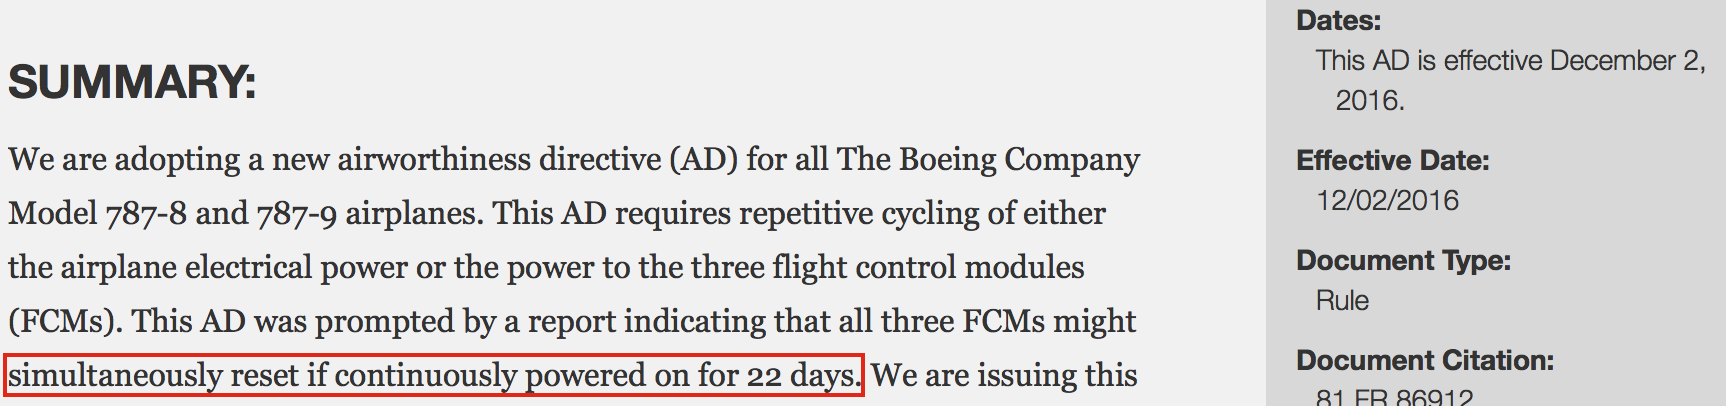
\includegraphics[width=1\framewidth]{dreamliner-bug-2016}};}
%   \end{tikzpicture}
% \end{frame}

% \begin{frame}[fragile]
%   \frametitle{The pernicious \texttt{int}}
%   Integers are represented either \emph{signed} or \emph{unsigned}
%   using a fixed number of \emph{bits}.

%   Let's try computing $127+1$, represented as 8bit signed integers.

%   \begin{uncoverenv}<2>
%   \begin{tikzpicture}
%     \matrix (m) [matrix of nodes,
%     nodes={minimum size=0.75cm, draw, anchor=center},
%     column sep=0pt,
%     ]
%     { $-2^7$ & $2^6$ & $2^5$ & $2^4$ & $2^3$ & $2^2$ & $2^1$ & $2^0$
%       \\};
%     \matrix (mfull) [matrix of nodes, below=0.2cm of m,
%     nodes={minimum size=0.75cm, draw, anchor=center},
%     column sep=0pt,
%     ]
%     { $0$ & $1$ & $1$ & $1$ & $1$ & $1$ & $1$ & $1$
%       \\};
%     \node [left=0.1cm of mfull]  {$127$};
%     \matrix (mone) [matrix of nodes, below=0.2cm of mfull,
%     nodes={minimum size=0.75cm, draw, anchor=center},
%     column sep=0pt,
%     ]
%     { $0$ & $0$ & $0$ & $0$ & $0$ & $0$ & $0$ & $1$
%       \\};
%     \node [left=0.1cm of mone] {$1$};
%     \node [above left=0.1cm and 0.3cm of mone.north west, anchor=center] {$+$};

%     \matrix (moops) [matrix of nodes, below=0.2cm of mone,
%     nodes={minimum size=0.75cm, draw, anchor=center},
%     column sep=0pt,
%     ]
%     { $1$ & $0$ & $0$ & $0$ & $0$ & $0$ & $0$ & $0$
%       \\};
%     \node [left=0.1cm of moops] {$-128$};
%     \node [above left=0.1cm and 0.3cm of moops.north west,
%     anchor=center] {$=$};
%     \node [right=0.1cm of moops] {(Probably)};
%   \end{tikzpicture}
%   \end{uncoverenv}
% \end{frame}

% \begin{frame}[fragile]
%   \frametitle{The pernicious \texttt{int}}
%   Let's go back and look at the Dreamliner numbers again.

%   \begin{equation*}
%     248\,\text{days} = 248 \times 24 \times 3600 \times 100 =
%     2142720000 \,\text{centiseconds}
%   \end{equation*}
%   \begin{equation*}
%     22\,\text{days} = 22 \times 24 \times 3600 \times 1000 =
%     1900800000 \,\text{milliseconds}
%   \end{equation*}


%   \begin{uncoverenv}<2>
%     \begin{equation*}
%       \log_2{2142720000} \approx 30.997
%     \end{equation*}
%   \begin{equation*}
%     \log_2{1900800000} \approx 30.824
%   \end{equation*}

%   Both of these failures are almost certainly due to \emph{integer
%     overflow} of a signed 32bit integer.
% \end{uncoverenv}
% \end{frame}

% \begin{frame}
%   \frametitle{Should you trust your calculation?}

%   Computing with real values provides a whole new class of ways to get
%   the wrong answer.

%   \begin{center}
%     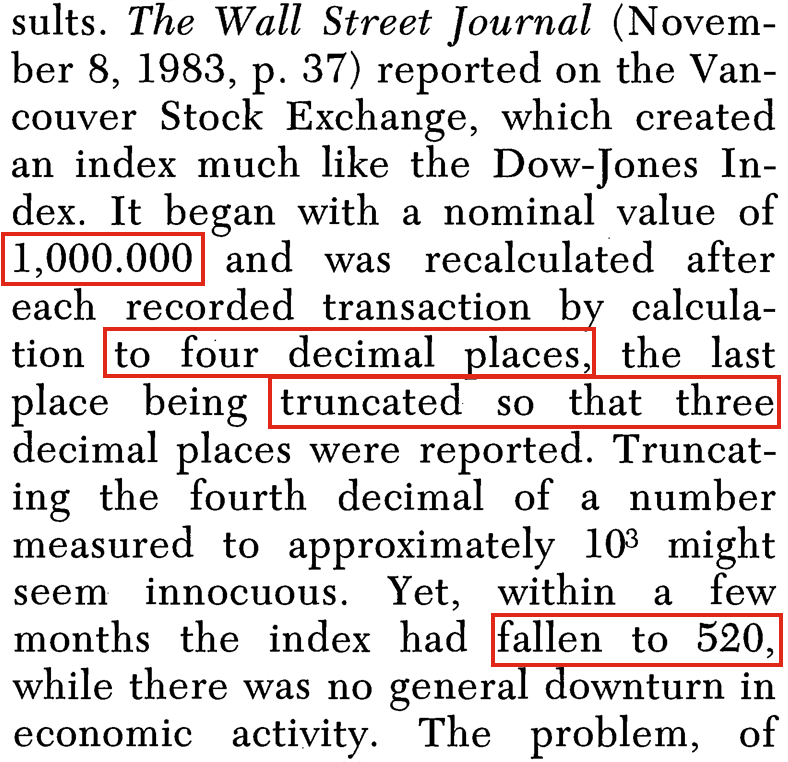
\includegraphics[height=0.6\textheight]{vancouver-index}
%   \end{center}
%   \begin{flushright}
%     {\scriptsize McCullogh \& Vinod, Journal of Economic Literature
%     37(2):633--665 (1999)}
%   \end{flushright}
% \end{frame}

% \begin{frame}
%   \frametitle{Floating point}
%   \begin{itemize}
%   \item The set of real numbers is uncountable, which presents
%     problems on a computer.
%   \item We typically approximate real numbers using \emph{floating
%       point}.
%   \item Scientific notation with a fixed number of
%     \emph{significant figures}
%   \end{itemize}
%   \begin{equation*}
%     1015323 = \underbrace{1.015323}_{\text{significand}} \times \underbrace{10}_{\text{base}}\!\!\!\!\!\!^{\overbrace{6}^{\text{exponent}}}
%   \end{equation*}
% \end{frame}

% \begin{frame}
%   \frametitle{Floating point}
%   \begin{itemize}
%   \item Behaviour implemented in CPUs standardised in IEEE 754
%   \item Specifies how to interpret bit patterns as floating point
%     numbers
%   \item Also specifies \emph{rounding} for calculations that result in
%     values that not exactly representable
%   \item Defines \emph{base} to be 2.
%   \end{itemize}
%   \begin{tabular}{c|ccc|c}
%     Precision & Sign & Exponent & Significand & Total bits \\
%     \hline
%     single    & 1    & 8        & 23          & 32         \\
%     double    & 1    & 11       & 52          & 64         \\
%   \end{tabular}
% \end{frame}

% \begin{frame}
%   \frametitle{Bit representation}
%   \begin{tikzpicture}
%     \node[rectangle,draw,inner sep=0pt, minimum width=1cm, minimum
%     height=0.5cm, anchor=west] at (0, 0) (sign) {sign};
%     \node[rectangle,draw,inner sep=0pt, minimum width=3cm, minimum
%     height=0.5cm, anchor=west] at (1cm, 0) (exp) {exponent};
%     \node[rectangle,draw,inner sep=0pt, minimum width=5cm, minimum
%     height=0.5cm, anchor=west] at (4cm, 0) (sig) {significand};
%     \node[left=0.1cm of sign.west] {$\text{val} = $};

%     \node[above=0cm of sign.north west] {32};
%     \node[above=0cm of sign.north east] {31};
%     \node[above=0cm of exp.north east] {23};
%     \node[above=0cm of sig.north east] {0};
%   \end{tikzpicture}
%   \begin{equation*}
%     f = \begin{cases}
%       \phantom{-}1.sssssssss_2 \times 2^{\text{exp}} & \text{sign} = 0\\
%       -1.sssssssss_2 \times 2^{\text{exp}} & \text{sign} = 1\\
%      \end{cases}
%    \end{equation*}
%    note ``hidden'' bit of precision, so
%    \begin{equation*}
%      f = (1 + \sum_{i=1}^{23} \text{val}_{i-1} * 2^{-i})\times 2^{\text{exp}}
%    \end{equation*}
% \end{frame}

% \begin{frame}
%   \frametitle{What about zero?}
%   \begin{itemize}
%   \item We need to play some tricks, and do so by stealing some bits
%     in the exponent.
%   \end{itemize}
%   \begin{center}
%     {\small
%       \begin{tabular}{c|c|c}
%         \multicolumn{2}{c|}{Exponent} & Value represented\\
%         Binary & Decimal & \\
%         \hline
%         $00000000_2$ & $0_{10}$ & Zero if significand is zero \\
%         $00000001_2$ & $1_{10}$ & $1.sssssssss_2 \times 2^{-126}$ \\
%         \dots & \dots & \dots \\
%         $01111111_2$ & $127_{10}$ & $1.sssssssss_2 \times 2^{-0}$ \\
%         $10000000_2$ & $128_{10}$ & $1.sssssssss_2 \times 2^{1}$ \\
%         \dots & \dots & \dots \\
%         $11111110_2$ & $254_{10}$ & $1.sssssssss_2 \times 2^{127}$ \\
%         $11111111_2$ & $255_{10}$ & $\infty$ if significand is zero\\
%       \end{tabular}
%     }
%   \end{center}
% \end{frame}

% \begin{frame}[fragile]
%   \frametitle{Almost all numbers are represented inexactly}
%   \begin{itemize}
%   \item Any irrational number ($\sqrt{2}, \pi, \dots$) is not exact in
%     floating point
%   \item But many rational numbers are also not (after all they are
%     countable, but still infinite).
%   \item In the same way that $1/3$ is $0.333\overline{33}_{10}$.
%   \item $0.1 = 0.0001100\overline{1100}_2$
%   \item The result of a calculation may not be the closest
%     representable number to the exact result!
%   \end{itemize}
%   \begin{center}
% \begin{minted}[fontsize=\small]{c}
% print 0.01f - (0.1f*0.1f); => -9.31323e-10
% \end{minted}
%   \end{center}
% \end{frame}

% \begin{frame}
%   \frametitle{Addition}
%   \begin{itemize}
%   \item How to add two numbers with different scales?
%     \begin{equation*}
%       1 \times 10^{6} + 2
%     \end{equation*}
%   \item \emph{Shift} so exponent is the same
%   \item add significands
%     \begin{align*}
%       1 \times 10^{6} + 2 &= \\
%       1 \times 10^{6} + 0.000002 \times 10^{6} &= \\
%       1.000002 \times 10^{6}
%     \end{align*}
%   \item What happens if there are not enough bits in the significand?
%   \end{itemize}
% \end{frame}

% \begin{frame}[fragile]
%   \frametitle{No associativity}
%   We expect that arithmetic operations \emph{associate}
%   \begin{equation*}
%     (a + b) - c = a + (b - c).
%   \end{equation*}

%   Floating point operations do not.

%     \begin{center}
%       \begin{onlyenv}<2>
% \begin{minted}[fontsize=\small]{c}
% print ((1f + 1e10f) - 1e10f);
% print (1f + (1e10f - 1e10f));
% \end{minted}
%       \end{onlyenv}
%     \end{center}
%     \begin{center}
%       \begin{onlyenv}<3>
% \begin{minted}[fontsize=\small]{c}
% print ((1f + 1e10f) - 1e10f); => 0.0f
% print (1f + (1e10f - 1e10f)); => 1.0f
% \end{minted}
%       \end{onlyenv}
%     \end{center}
% \end{frame}

% \begin{frame}[fragile]
%   \frametitle{No distributivity}
%   We expect that multiplication \emph{distributes} over addition
%   \begin{equation*}
%     (a + b)*c = a*c + b*c
%   \end{equation*}

%   Again, this does not occur in floating point.

%   \begin{center}
%     \begin{uncoverenv}<2>
% \begin{minted}[fontsize=\small]{c}
% float a = 1234.5678f;
% float b = 1.2345678f;
% float c = 3.3333333f;
% print (a+b)*c; => 4119.3413f
% print (a*c) + (b*c); => 4119.3408f
% \end{minted}
%     \end{uncoverenv}
%   \end{center}
% \end{frame}

% \begin{frame}
%   \frametitle{Sensitivity of numerical algorithms}
%   \begin{itemize}
%   \item The study of the accuracy and stability of numerical algorithms is as old
%     as computers.
%   \item Concerned with how errors propagate through an algorithm.
%   \item A core concept here is \emph{conditioning}.
%   \end{itemize}

%   Intuitively, conditioning tells us how sensitive the output of a
%   function is to small changes in its inputs.
% \end{frame}

\end{document}
